
\chapter{Spatial Sampling Designs and Analysis}

\section{Ecological Inference and Field Sampling}

Like all scientists, ecologists seek to understand the world through an iterative process of reduction and subsequent composition.  This typically involves decomposing a complicated phenomenon into smaller processes that can be studied experimentally and in isolation (\textit{reduction}), and then some effort to identify how much of the original phenomenon can be explained via those mechanisms that have been identified via previous experiments (\textit{composition}).  However, ecologists are faced with many unique challenges in this scientific process including:

\begin{enumerate}
    \item \textit{Multicausality}\index{multicausality}:  ecologists seek to predict a wide range of dynamics, including individual behavior, population/community dynamics, and ecosystem function (to name a few).  However, most ecological variables are impacted by many other variables simultaneously, and those in turn are impacted by many others.  Analysts can represent these causal mechanisms using a \myindex{causal map} \cite{pearl_causal_2009}, and the causal maps associated with real-world ecosystems are very complex relative to a controlled experiment in classical mechanics (e.g., a pendulum operating under drag and gravity) or chemistry (e.g., reactions occurring under well-mixed concentrations and known physical principles);  
    
    \item \textit{{Tapering effects}}\index{tapering effects}:  most ecological problems are defined at a level of organization that involves hundreds or thousands of mechanisms that have been observed in isolated settings.  For example, the tendency for communities to persist through time is called \myindex{community regulation}, and modern coexistence theory seeks to enumerate and categorize the many ecological processes that promote community persistence into a smaller set of mathematical expressions \cite{ellner_expanded_2019}.  However, essentially all potential mechanisms are likely to have some non-zero (if vanishingly small) role in dynamics for a given system. If we plotted the importance (e.g., variance explained) by different possible measurements or mechanisms in rank order from most to least important, this plot would likely have a longer tail than other types of science (this phenomenon is called \myindex{tapering effects} \cite{burnham_multimodel_2004}).  This contrasts, for example, with classical mechanics (studied in physics) where a small number of mechanisms can describe essentially all properties of solid objects and their movement within space;     

    \item \textit{Lack of experimental control}:  finally, ecologists often address questions at a scale that does not permit experimentation, either because it would be unethical (i.e., experiments on humans as elements of an ecosystem without their consent), impractical (i.e., multi-generational experiments on long-lived populations), technically impossible (i.e., experimental control of individual behavioral mechanisms in complex organisms), or context-dependent (i.e., require repeating experiments for every described species and habitat).  In these cases, ecologists must instead use insights derived from experiments in analogous systems and identify dominant mechanisms based on incomplete information from lower levels of organization.
\end{enumerate}
These challenges all complicate the traditional scientific process of reduction and composition when applied to ecological systems.  

For these three reasons (among others), applied ecologists have adopted a scientific process that prioritizes repeated, direct measurements of important variables in real-world ecosystems (\index{ecological monitoring}\textit{ecological monitoring}) that can directly inform the management of real-world systems.  These ecological monitoring programs (e.g., the International Long-Term Ecological Research Network \cite{vanderbilt_international_2017}) then provide data sets that are described using a shared set of dynamical models, and ecological theory seeks in part to define this set of shared dynamical models.  However, the design and analysis of ecological monitoring programs comes with additional challenges.  In the following, we specifically address the following topics related to the design and analysis of ecological monitoring programs:

\begin{enumerate}
    \item \textit{Spatial integration}\index{spatial integration}:  how to estimate a spatially integrated total (i.e., total abundance) by fitting a spatial model to local measurements;

    \item \textit{Non-ignorable sampling designs}:  how to analyze data that arise non-experimentally, and where the probability of data being available may be correlated with the variable of interest;

    \item \textit{Muli-stage sampling}:  how to analyze data that involves multiple levels of subsampling.
\end{enumerate}
These problems all involve some background in sampling theory, and we note that other textbooks provide an alternative perspective on these and other topics from a design-based perspective \cite{cochran_sampling_1977}.  

\section{Spatial Integration and Weighting} \label{sec:Chap6_spatial_integration}

Ecologists often seek to estimate the average or total value for a given variable when aggregating across space.  Many governments mandate a change in regulation based on the aggregated total for a system variable.  For example, environmental agencies might want to maintain a population sizes for the endangered North Atlantic right whale (\textit{Eubalaena glacialis}) above some threshold, or ensure that wetland habitats maintain a total area above some target.  As we will see, calculating this total leads to several different algorithms for spatial integration, and each is suitable for analyzing different ecological variables, attributes, or processes\footnote{See https://github.com/james-thorson/Spatio-temporal-models-for-ecologists/Chap\_6 for code associated with this chapter.}.  

To illustrate these principles, we introduce a data set of samples of air pollution compiled by AirNow \cite{timothy_raw_2004}.  AirNow includes daily measurements of particles suspended in the atmosphere that are smaller than a specified size (PM2.5 and PM10) as well as ozone, using standardized measurement systems that are approved by the United States Environmental Protection Agency.  We specifically downloaded 8-hour average \myindex{ozone concentrations} in southeastern and mid-Atlantic states (Florida through New York)\footnote{obtained from the EPA Outdoor Air Quality Data center on July 19, 2022.} and note that the EPA in 2015 defined a standard for human ozone exposure of 0.07 parts per million (ppm).  We then combine these air pollution measurements with global estimates of human population density at 1-degree resolution available in 2000, 2005, 2010, 2015, and 2020, using the UN WPP-Adjusted Population Density, v4.11 \cite{center_for_international_earth_science_information_networkciesin_gridded_2016}\footnote{accessed from the NASA Socioeconomic Data and Applications Center on July 22, 2022.}.   

We first fit a spatial linear mixed model to ozone measurements occurring on July 1, 2019, using the SPDE method to define the distribution of a spatial variable \( \mathbf{\omega} \) and using population density as a covariate:

\begin{equation} \label{eq:Chap6_ozone}   
\begin{gathered} 
    \log(\mathbf{\mu}) = \beta_0 + \mathbf{A \omega} + \beta_1 \mathbf{d}  \\
    \mathbf{\omega} \sim \mathrm{MVN}( \mathbf{0, Q}^{-1} ) \\
    y_i \sim \mathrm{Gamma}( \sigma^{-2}, \mu_i \sigma^2 )
\end{gathered}
\end{equation}
where \( \mathbf{Q} \) is the precision matrix defined using the SPDE method, \(\mathbf{\omega}\) is the vector of spatial random effects at each SPDE vertex, \( \mathbf{A} \) is the matrix representing bilinear interpolation from SPDE vertices to the locations of data, \(\mathbf{d}\) is the vector of population density at each sample, and \(\mathrm{Gamma}\) is a gamma disribution with shape \( \sigma^{-2} \) and scale \(\mu_i \sigma^2\) where \(\sigma\) is the estimated coefficient of variation.  

\begin{figure}[!ht]
    \caption[Predicted and observed ozone concentrations]{Measured ozone concentrations (top-left panel) along with the SPDE mesh arising from a uniform grid overlaid on the spatial domain, the predicted ozone densities (top-right panel, in ppm), predictive standard errors (bottom-left, in ppm), and human population density in 2020 extracted from a global data product with 1-degree resolution (bottom-right panel and plotted on log-scale).}
    \centering
    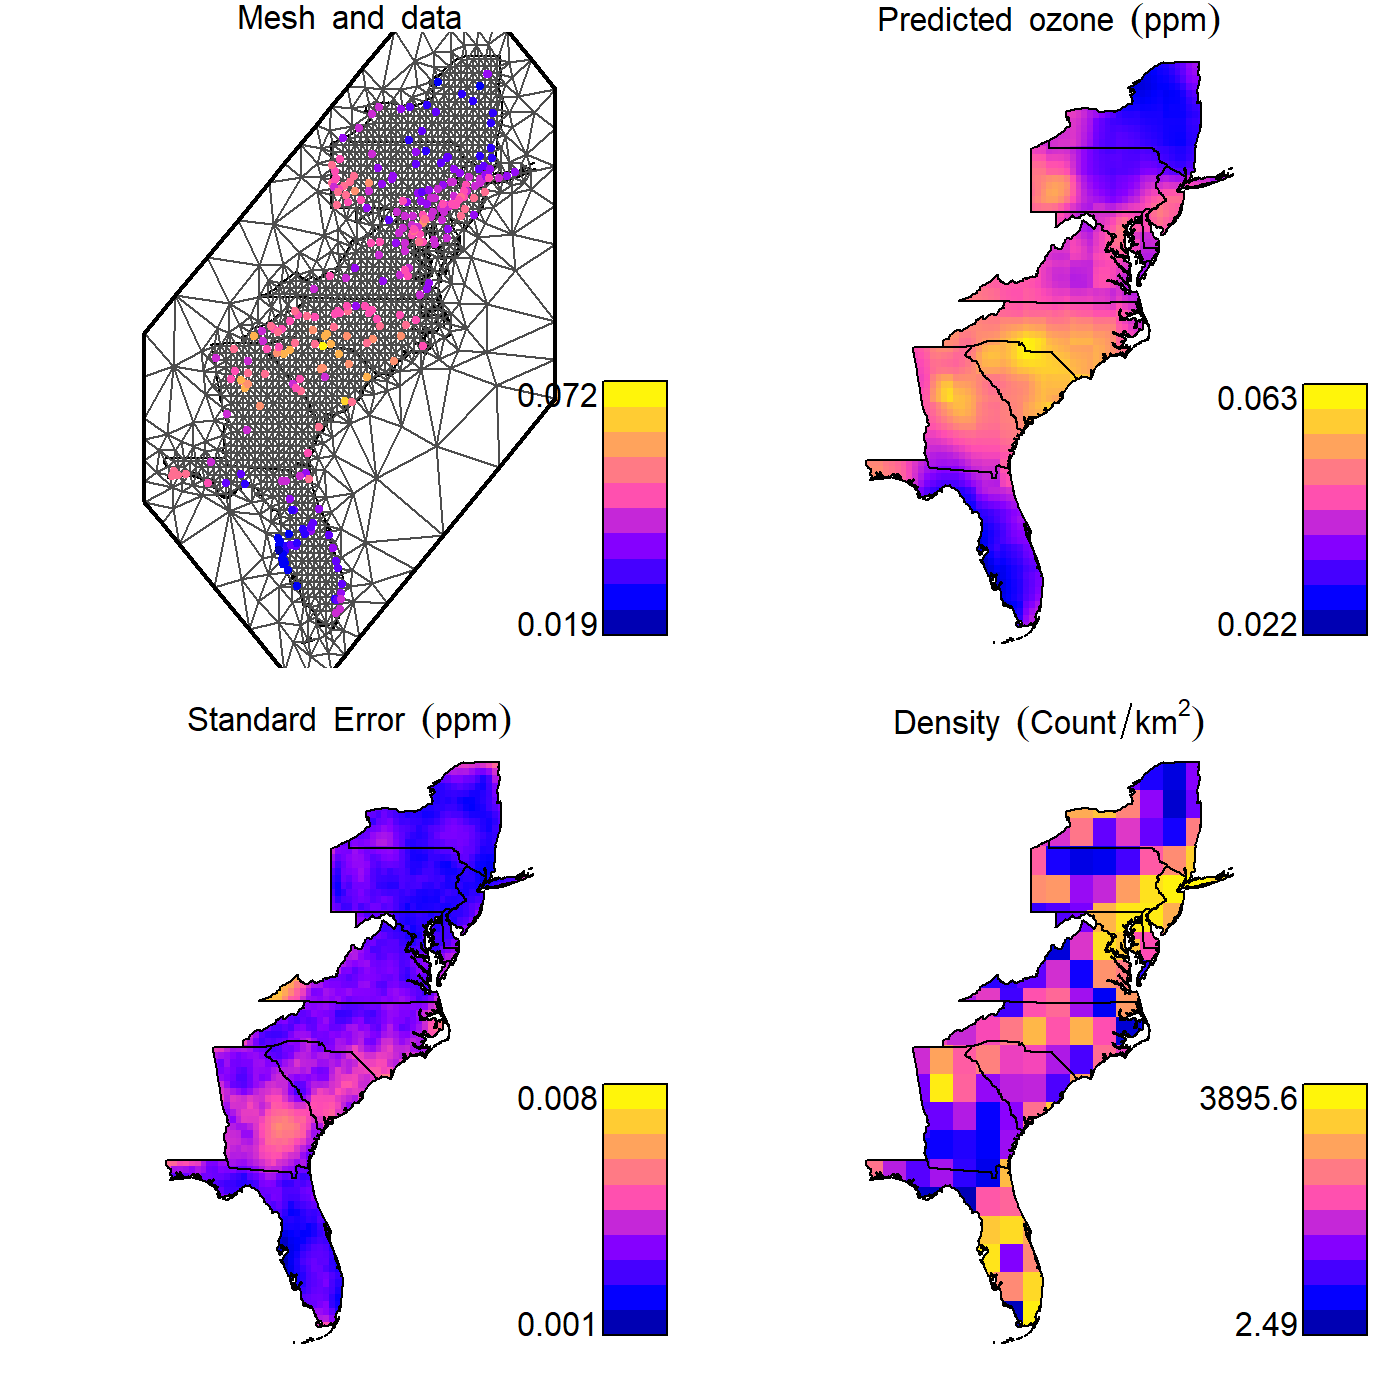
\includegraphics[width=5.5in]{Chap_6/Mapped_ozone.png}
    \label{fig:Chap6_Mapped_ozone}
\end{figure}

\subsection{Estimating Uncertainty in Derived Quantities} \label{sec:Chap6_sample_joint_precision}

This model can then be used to predict ozone concentrations at any other location \(s \in \mathcal{D} \) within the spatial domain \(\mathcal{D}\) where covariate \(d(s)\) is also known.  These predictions therefore define a function \( \mu(s) \) over that same spatial domain and we start by mapping the value \( \mu(s) \) at evenly spaced locations (Fig. \ref{fig:Chap6_Mapped_ozone}).  In general, we will also want to calculate, visualize, and communicate our uncertainty when predicting \( \hat\mu(s) \).  Recall from Eq. \ref{eq:Chap2_joint_precision}) that we can construct the \myindex{joint precision matrix} from the inner and outer Hessian matrices, as well as the gradient of predicted random effects given fixed effects (the outer Jacobian matrix).  This joint precision \(\mathbf Q_{joint}\) is often sparse, due to the sparsity of the inner Hessian matrix when using a sparse precision matrix (i.e., a CAR, SAR, or SPDE method to define spatial autocorrelation).  We could further calculate the joint covariance, \( \mathbf V_{joint} = \mathbf Q_{joint}^{-1} \), although taking the matrix inverse will then typically result in a dense covariance matrix, so computing the joint covariance \(\mathbf V_{joint} \) is computationally infeasible for large models.

We then approximate the uncertainty in fixed and random effects in two ways:
\begin{enumerate}
    \item \textit{Sample-based}: we can estimate uncertainty by taking samples of both fixed and random effects while assuming that they are normally distributed with mean equal to their empirical Bayes prediction (for random effects) and maximum likelihood estimates (for fixed effects) and variance of their inverse precision \(\mathbf{Q}_{joint}\).  Given that \(\mathbf Q_{joint}\) is often sparse, we specifically use a custom R-function \colorbox{backcolour}{rmvnorm\_prec} to generate multivariate-normal samples from this precision matrix without having to compute or store the matrix inverse in memory (Code \ref{code:Chap6-rmvnorm-prec}).  This code specifically uses the \colorbox{backcolour}{Matrix} package \cite{bates_matrix_2023} to decompose a sparse precision matrix \( \mathbf{Q = P}^t \mathbf{L} \mathbf{L}^t \mathbf{P} \), where \(\mathbf{L}\) is a sparse lower-triangle matrix and \(\mathbf{P}\) is a permutation matrix.  This generalizes the Cholesky decomposition (see Section \ref{sec:Appendix_Cholesky}) for efficient use with sparse matrices by including a permutation matrix \( \mathbf{P}\). This decomposition then allows us to use \colorbox{backcolour}{Matrix} to efficiently calculate \( \mathbf{z}^{\ast} = \mathbf{P}^t (\mathbf{L}^t)^{-1} \mathbf{z} \) where \(\mathbf{z}\) are independent samples from a standard normal distribution, and \( \mathbf{z}^{\ast} \sim \mathrm{MVN}(\mathbf{0,Q}_{joint}^{-1}) \) \cite{rue_gaussian_2005};
    
    For each sample from the joint precision matrix, we then plug these into our calculation of \( \mu \) (using Eq. \ref{eq:Chap6_ozone}).  We specifically do this using custom function \colorbox{backcolour}{sample\_var} (Code \ref{code:Chap6-sample-var}) by passing the vector new fixed and random effects to the compiled TMB object \colorbox{backcolour}{obj\$report}, so that we can use the same code as was used during parameter estimation.  We can use this function \colorbox{backcolour}{sample\_var} generically for any fitted TMB model (e.g., in Code \ref{code:Chap6-demonstrate-sample-var}).  We then interpret the standard deviation across samples as a sample-based approximation to the predictive standard error;  

    \item \textit{Generalized delta method}: alternatively, we can can define a function \(\phi\) for calculating a derived quantity, in this case \( \mu_i = \phi(\theta,\epsilon) \), where \( \theta \) and \( \epsilon \) are fixed and random effects, respectively.  We then calculate the matrix of gradients of this function \( \phi \) with respect to fixed and random effects, \( \mathbf G = \nabla \phi \), and then calculate the covariance of derived quantities as \( \mathbf{ G Q}_{joint}^{-1} \mathbf G^t \).  
\end{enumerate}
The generalized delta method requires calculating gradients for each derived quantity, and thus becomes computationally expensive when calculating the standard error for a large number of quantities (e.g., predicting ozone concentrations at a high spatial resolution).  By contrast, the sample-based method approximates the uncertainty using a specified number of samples, and therefore introduces some sampling error in the calculated standard errors.  When to use each of these two approximations depends somewhat on context, including the number of random effects and the need for a precise calculation.  

\lstset{style=Rcode}
\lstinputlisting[language=R, label=code:Chap6-rmvnorm-prec, caption=R function \colorbox{backcolour}{rmvnorm\_prec} demonstrating how to efficiently sample from a multivariate normal distribution when supplying a sparse precision matrix., captionpos=t]{Shared_functions/rmvnorm_prec.R}

\lstset{style=Rcode}
\lstinputlisting[language=R, label=code:Chap6-sample-var, caption=R function \colorbox{backcolour}{sample\_var} demonstrating how to efficiently sample from the joint precision matrix of fixed and random effects estimated by TMB using a mixed-effects model., captionpos=t]{Shared_functions/sample_var.R}
    
\lstset{style=Rcode}
\lstinputlisting[language=R, label=code:Chap6-demonstrate-sample-var, firstline=99, lastline=107, caption=R code demonstrating interface to efficiently sample from joint precision of fixed and random effects., captionpos=t]{Chap_6/Ozone_example.R}

Using the sample-based method to approximate and map the standard errors for ozone concentrations, this model predicts concentrations approaching 0.06 ppm (but still below the 0.07 ppm EPA standard) near Atlanta and along the boundary of North and South Carolina, with the lowest concentrations in central Florida and northern New York (Fig. \ref{eq:Chap6_ozone}).  We also see comparatively low standard errors throughout the spatial domain.

\subsection{Expansion Weights} \label{sec:Chap6_expansion_weights}

Ecological inference often involves integrating an estimated function across some spatial domain \( s \in \mathcal{D} \).

\begin{equation} \label{eq:Chap6_integral}
    \hat{y} = \int_{\mathcal{D}} \hat\mu(s) w(s) \mathrm{d}s
\end{equation}
where \(w(s)\) is a expansion term when calculating this integral.  In practice, this integral is typically approximated using \myindex{Monte Carlo integration} \cite{wadoux_uncertainty_2023} (Table \ref{tab:Chap2_integration}) by defining a set of \(n_g\) \myindex{integration points}, \( g \in \{1,2,...,n_g\}\) where \( s_g \in \mathcal{D}\).  This then replaces the integral in Eq. \ref{eq:Chap6_integral} with a summation:

\begin{equation} \label{eq:Chap6_sum}
   \hat{y} = \sum_{g=1}^{n_g} \hat\mu(s_g) w_g a_g 
\end{equation}
where \( a_g \) represents the area associated with each integration point \(s_g\).  These integration points can be chosen in many ways, perhaps with higher densities in areas of particular interest, but in the following, we will generally define a set of evenly spaced grid cells, so that the same locations can be used for plotting and spatial integration.

We highlight four different weighting methods that define the weight \(w_g\) and area \(a_g\) associated with each integration point, noting that other methods will arise in practice:
\begin{itemize}
    \item \textit{Sample weighted total}:  most simply, an analyst might calculate density function \(\hat \mu\) at the set of locations where samples were taken.  This specifies the same number of integration points and samples \(n_g = n_i\) and \(s_g = s_i\), and presumably also an equal area assigned for each integration point \( w_g=a_g=1 \).  Sample weighting is useful, e.g., when sampling locations were chosen as part of a panel design, they were chosen at locations that are somehow representative of the sampled variable, or otherwise have specific ecological or stakeholder interest;  

    \item \textit{Area-weighted average}: instead, an analyst might calculate the total over some irregularly shaped domain \(\mathcal{D}\).  In this case, quadrature points near a boundary might represent a smaller area than quadrature points that are entirely enclosed by the domain, such that \(a_g\) varies among integration points while \(w_g=1\) for all of them;

    \item \textit{Covariate-weighted average}:  in other cases, an analyst might weight the estimated variable \(\mu\) based on a quantity that is assumed to be known without error.  For example, to calculate total ozone exposure, we might calculate the weighted average of predicted ozone concentrations \(\hat\mu(s_g)\), weighted by human population densities \(d(s_g)\) such that \(w_g = \frac{d(s_g)}{\sum_{g=1}^{n_g} d(s_g)}\);   

    \item \textit{Multivariate-weighted average}: finally, it might be helpful to use covariate-weighting but using other modeled variables in place of a fixed covariate for weighting \(w_g\).  For example, an analyst might seek to measure the average body size of individuals in a population.  To do so, they could jointly model a measurement of body size \(B(s)\) as well as population density \(N(s)\) at different locations \( s \in \mathcal{D} \).  The analyst could then calculate the average body size for each integration point \(\hat{\mu}_g = B(s_g)\), weighted by the proportion of numerical abundance \(w_g = \frac{a_g N(s_s)}{\sum_{g=1}^{n_g} a_g N(s_g)} \) associated with that location \cite{gruss_developing_2019}.  

\end{itemize}
In the following, we contrast the first three weighting methods when applied to the ozone concentration example.  However, we first introduce a potential source of bias called \textit{retransformation bias}, and also introduce a practical solution called \textit{epsilon bias-correction}.

\subsection{Epsilon Bias-correction}

First recall that hierarchical models treat random effects as random variables that follow some specified distribution, and that the marginal likelihood is calculated by integrating across the value of random variables (Section \ref{sec:Chap2_deriving_random_effects}).  For illustration, we introduce a single random variable \(\epsilon\) but seek to estimate a variable \( Z = \phi(\epsilon) \) that is calculated via some transformation \(\phi\) that might be nonlinear.  To illustrate, let's imagine that \(\epsilon\) follows a normal distribution and is then exponentiated, and we seek an unbiased pointwise estimator \(\hat Z\), defined as the expected value for the distribution \(Z\):

\begin{equation}
\begin{gathered}
    \epsilon \sim \mathrm{Normal} (\mu, \sigma^2) \\
    Z = e^{\epsilon} \\
    \hat Z = \E(Z)
\end{gathered}
\end{equation}
In this simple case, we know that \( Z \) follows a lognormal distribution, and we can calculate the mean of this lognormal distribution analytically \( \hat Z = e^{\mu + 0.5\sigma^2} \), where an unbiased estimator will have this same value. However, the simplest ``plug-in" estimator involves estimating the mode of the random effect, \( \hat \epsilon = \mu \), and then plugging that value into the transformation, such that \( \hat Z = e^{\mu} \).  This plug-in estimator obviously has a negative bias relative to the known expected value \(\E(Z)\).  This bias in the plug-in estimator is called \myindex{retransformation bias}.  

The plug-in estimator may also be biased due to \myindex{posterior skewness bias}.  To see this, imagine that we replace the normal distribution \( \epsilon \sim \mathrm{Normal} (\mu, \sigma^2) \) with a shape-scale parameterization of the Gamma distribution \( \epsilon \sim \mathrm{Gamma} (k, \theta) \) and assuming that \(k \geq 1\) for illustration purposes.  Let us further imagine that we want an unbiased estimator for \(\hat Z = \E(\epsilon)\), i.e., using an identity link instead of the previous log-link function.  In this case, the plug-in estimator involves calculating the mode of the random effect, \( \hat \epsilon = (k-1)\theta \) and then calculates \( \hat Z = (k-1)\theta \).  However, the mean of the gamma distribution is actually \( \E(\epsilon) = k \theta \), where the mean is greater than the mode due to the positive skewness of the Gamma distribution when \(k \geq 1\).  We can see that the skewness of the random effect \(\epsilon\) contributes to a bias when using the plug-in estimator to calculate the expected value for some transformation \(\E(\phi(\epsilon))\).  

From these thought-experiments, we can deduce that the magnitude of bias for the plug-in estimator increases whenever:
\begin{enumerate}
    \item random effect \(\epsilon\) has a large standard deviation.  In a mixed effects model, this will occur when the empirical Bayes prediction for a random effect used in the calculation of a given derived quantity has a large standard error; or

    \item available data result in an estimate of random effects that has non-zero skewness; and

    \item the function used to compute the derived quantity is highly nonlinear with respect to random effects.  The bias therefore arises in generalized linear mixed models for all link functions except the identity link.
\end{enumerate}
Many ecological applications for spatial and spatio-temporal models have a response variable that is constrained to be positive (such that analyses often specify a nonlinear link function like the log-link), and also have limited data (hence having large imprecision for estimated random effects).  Furthermore, many population-dynamics models resulted in non-zero skewness for random effects.  We therefore conclude that the plug-in estimator will be biased in many practical applications.  

To correct for plug-in estimator bias when using the Laplace approximation, we therefore introduce the \myindex{epsilon bias-correction estimator}. Skipping the derivation \cite{thorson_implementing_2016,tierney_fully_1989}, recall that the Laplace approximation involves defining the joint log-likelihood of fixed \( \theta \) and random effects \( \epsilon \) given data \(y\), \( f( \theta, \epsilon; y ) \), such that the marginal likelihood \( \mathcal{L}(\theta;y) = \int e^{f(\theta,\epsilon;y)} \mathrm{d}\epsilon \).  We then augment the joint log-likelihood by including an additional term, and calculate the Laplace approximation of this augmented likelihood \(\mathcal{L^*}(\theta, \delta; y)\):
\begin{gather} \label{eq:Chap6_epsilon_method}
    f^*( \theta, \epsilon, \delta; y ) = f( \theta, \epsilon; y ) - \delta \phi(\theta,\epsilon) \\
    \mathcal{L^*}(\theta, \delta; y) = \int e^{f^*(\theta,\epsilon,\delta;y)} \mathrm{d}\epsilon \\
    \E(\phi(\theta,\epsilon)) = \hat \phi(\theta,\epsilon) = \frac{\partial}{\partial \delta} \log(\mathcal{L^*}(\theta, \delta; y))|_{\delta=0}
\end{gather}
where we generalize the previous notation by noting that derived quantity \(\phi(\theta,\epsilon)\) might be a nonlinear function of both fixed and random effects.  We then evaluate the gradient of the log-marginal augmented likelihood with respect to \( \delta \) evaluated at \( \delta=0\). This gradient is then a high-quality approximation to the unbiased estimator for the derived quantity \(\phi(\theta,\epsilon)\).

When applying the epsilon estimator to a single random effect (e.g., Eq. \ref{eq:Chap6_epsilon_method}), it can be decomposed into the following three terms:

\begin{equation} \label{eq:Chap6_epsilon_decomposition}
\begin{gathered}
    \hat{\phi}(\epsilon) = \underbrace{\phi(\hat \epsilon)}_{\text{Plug-in}} - \underbrace{\frac{1}{2} \frac{\phi''(\hat \epsilon)}{f''(\hat \epsilon)}}_{\text{Nonlinearity in }\phi} - \underbrace{\frac{1}{2}  \phi'(\hat \epsilon)  \frac{f'''(\hat \epsilon)}{f''(\hat \epsilon)^2}}_{\text{Skewness in f}}
\end{gathered}
\end{equation}
where \(\phi''(\cdot)\) is the second derivative of transformation \(\phi(\cdot)\) (which is zero when \(\phi\) is linear, i.e., using an identity link function), \(f''(\hat \epsilon)\) is the second derivative of the joint likelihood (i.e., the Hessian, such that \(\frac{1}{f''(\hat \epsilon)}\) is the variance of \(f\)), and \(f'''(\hat \epsilon)\) is the third derivative of the joint likelihood and therefore measures skewness.  The second term (labeled \textit{Nonlinearity in g}) accounts for the issues raised in the lognormal example, where the variance in random effects (\(\frac{1}{f''(\hat \epsilon)}\)) and the nonlinearity in the transformation (\(\phi''(\hat \epsilon)\)) combine to cause bias.  The third term (labeled \textit{Skewness in f}) is calculated from the third-derivative of the joint log-likelihood and therefore corrects for skewness.  

Alternatively, it is feasible to correct for bias resulting from nonlinear transformations and skewness by taking samples from the estimated distribution of random effects, transforming these samples, and taking the mean of these transformed values.  For example, this sample-based method occurs naturally when using \textit{Markov Chain Monte Carlo} to sample from a posterior distribution, and Bayesian hierarchical models therefore provide a natural way of computing the posterior mean for any derived quantity.  However, it is difficult in general to obtain samples from the joint log-likelihood \(f\) for use in calculating \( \phi(\theta,\epsilon) \) for large and nonlinear hierarchical models; this is precisely why we instead introduced the Laplace approximation in the previous chapters.  Alternatively, we saw in Sec \ref{sec:Chap6_sample_joint_precision} that we can take samples from a multivariate normal approximation to the joint log-likelihood (Eq. \ref{eq:Chap2_joint_precision}).  This multivariate normal approximation corrects for the second term of Eq. \ref{eq:Chap6_epsilon_decomposition}.  However, the multivariate-normal distribution has zero skewness, so this multivariate-normal approximation does not account for the skewness of random effects that is included as the third term of Eq. \ref{eq:Chap6_epsilon_decomposition}.  We therefore expect samples from the joint precision (e.g., using Eq. \ref{eq:Chap2_joint_precision}) to perform poorly when the random effects have substantial skewness.  

We demonstrate these concepts for our example where \(\epsilon\) is normally distributed and \( Z=e^{\epsilon}\), and add code to calculate the epsilon-correction manually or sample directly from the known distribution in a TMB function (Code \ref{code:Chap6-TMB-epsilon}).  In this case, we manually add the additional term \colorbox{backblue}{delta(0) * Z} to the joint negative log-likelihood (see the first line of Eq. \ref{eq:Chap6_epsilon_method}).  We also compare this manual implementation with the automated version that can be accessed by outputting any variable using the \colorbox{backblue}{ADREPORT} function in TMB, and then calling the function \colorbox{backcolour}{sdreport(..., bias.correct=TRUE)} in R (Code \ref{code:Chap6-R-epsilon}).  This code allows us to explore either normal or gamma distributions, using either an identity, square-root, or exponential transformation, and compares the epsilon estimator against the mean of samples drawn from the known distribution. 

\lstset{style=TMBcode}
\lstinputlisting[language=c++, label=code:Chap6-TMB-epsilon, caption=TMB code demonstrating how the epsilon bias-correction estimator is implemented., captionpos=t]{Chap_6/epsilon_estimator.cpp}

\lstset{style=Rcode}
\lstinputlisting[language=R, label=code:Chap6-R-epsilon, firstline=9, lastline=38, caption=R code demonstrating the equivalence of the manual and automated implementation of the epsilon bias-correction estimator., captionpos=t]{Chap_6/Epsilon_demo.R}

Finally, we compare the plug-in and epsilon bias-corrected estimators with the known expectation for this simple lognormal case (Fig. \ref{fig:Chap6_retransformation_bias}), and this shows that the epsilon estimator is very close to (but not quite) identical to the known value.  This epsilon bias-correction estimator therefore serves as a generic approach to deal with retransformation and skewness bias without requiring samples from the joint log-likelihood, either using MCMC at high computational cost or a multivariate-normal approximation that ignores the skewness of random effects.  Despite its convenience, however, we note that calculating the sum across a set of random effects and including them in the calculation of a joint likelihood often causes these random effects to no longer be conditionally independent (see the graphical representation of sparsity from Section \ref{sec:Chap2_Hessian_sparsity}).  Therefore, the epsilon estimator will sometimes break the sparsity of the inner Hessian matrix, and thereby require long computation when running \colorbox{backcolour}{sdreport(..., bias.correct=TRUE)} in R.  We therefore use it for only those variables where it is most important that a high accuracy bias-corrected estimator be used. In other cases where a lower accuracy approximation is sufficient (e.g., for high-resolution maps of results), we then tend to revert to the multivariate-normal approximation knowing that it will ignore the skewness of random effects.   

\begin{figure}[!ht]
    \caption[Retransformation bias and the epsilon bias-correction estimator]{The density for a normally distributed random variable (top panel), and the lognormal density that arises after it is exponentiated (bottom panel), showing the analytical calculation of it's expected value (which is the true value for an unbiased estimator), the plug-in estimator (which is negatively biased), and the epsilon bias-corrected estimator (which has very minimal bias).}
    \centering
    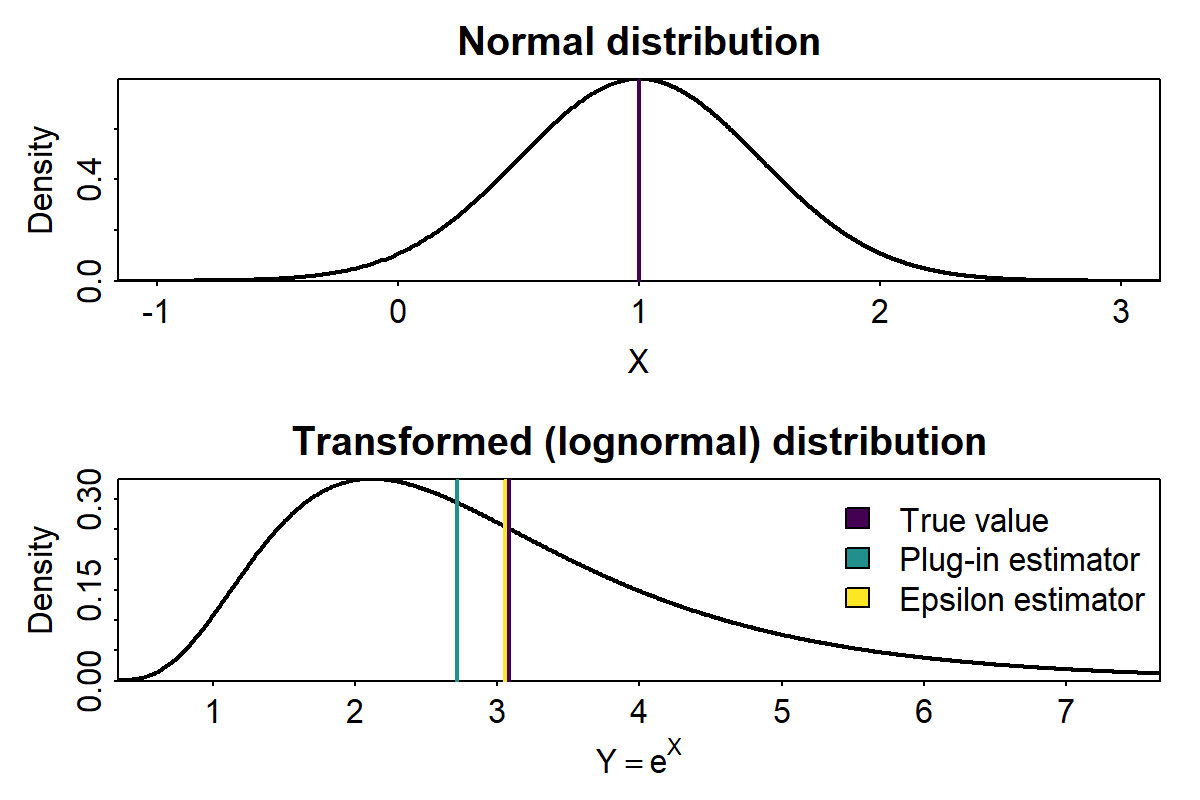
\includegraphics[width=5.5in]{Chap_6/Retransformation_bias.png}
    \label{fig:Chap6_retransformation_bias}
\end{figure}

We next return to a more complicated example of retransformation bias and epsilon bias-correction.  In section \ref{sec:Chap6_spatial_integration}, we defined a log-linked linear predictor involving a spatial variable and a single covariate (Eq. \ref{eq:Chap6_ozone}) and then calculated the total \( \hat y \) by summing across the exponentiated value of the linear predictor (Eq. \ref{eq:Chap6_sum}).  The plug-in estimator \(y^*\) involves taking empirical Bayes predictions of random effects \(\hat\omega\), and plugging them directly into the formula for spatial expansion (Eq. \ref{eq:Chap6_sum}):

\begin{equation}
   y^* = \sum_{g=1}^{n_g} w_g a_g e^{\hat\beta_0 + \mathbf{A \hat\omega} + \hat\beta_1 \mathbf{d}}  
\end{equation}
where \( \hat\omega \) are predicted as the mode of the joint likelihood given the estimated value of fixed effects.  However, \( \omega\) are estimated as random effects, and we would like to calculate \(\hat y\) as the expected value across these random variables:

\begin{equation}
    \hat{y} = \E\left(\sum_{g=1}^{n_g} w_g a_g e^{\hat\beta_0 + \mathbf{A \omega} + \hat\beta_1 \mathbf{d}} \right)
\end{equation}
We therefore calculate the sample-weighted, area-weighted, and population-density-weighted average ozone, either using the plug-in or epsilon bias-correction estimators.  In this example (Fig. \ref{fig:Chap6_totals}), the sample-weighted average is slightly higher than either area or population-density weighted averages.  As expected the epsilon bias-correction results in a slight increase for each estimator, where this positive correction results because the derivative of the transformation (in this case, exponentiation) is positive.    

\begin{figure}[!ht]
    \caption[Alternative weighting for average ozone concentration]{The sample weighteed (Y1), area-weighted (Y2), or population-density-weighted (Y3) average 8-hour ozone concentration on July 1, 2019 in parts per million using the plug-in estimator, or showing the same weighting methods but using the epsilon bias-correction estimator (Z1, Z2, and Z3 respectively).}
    \centering
    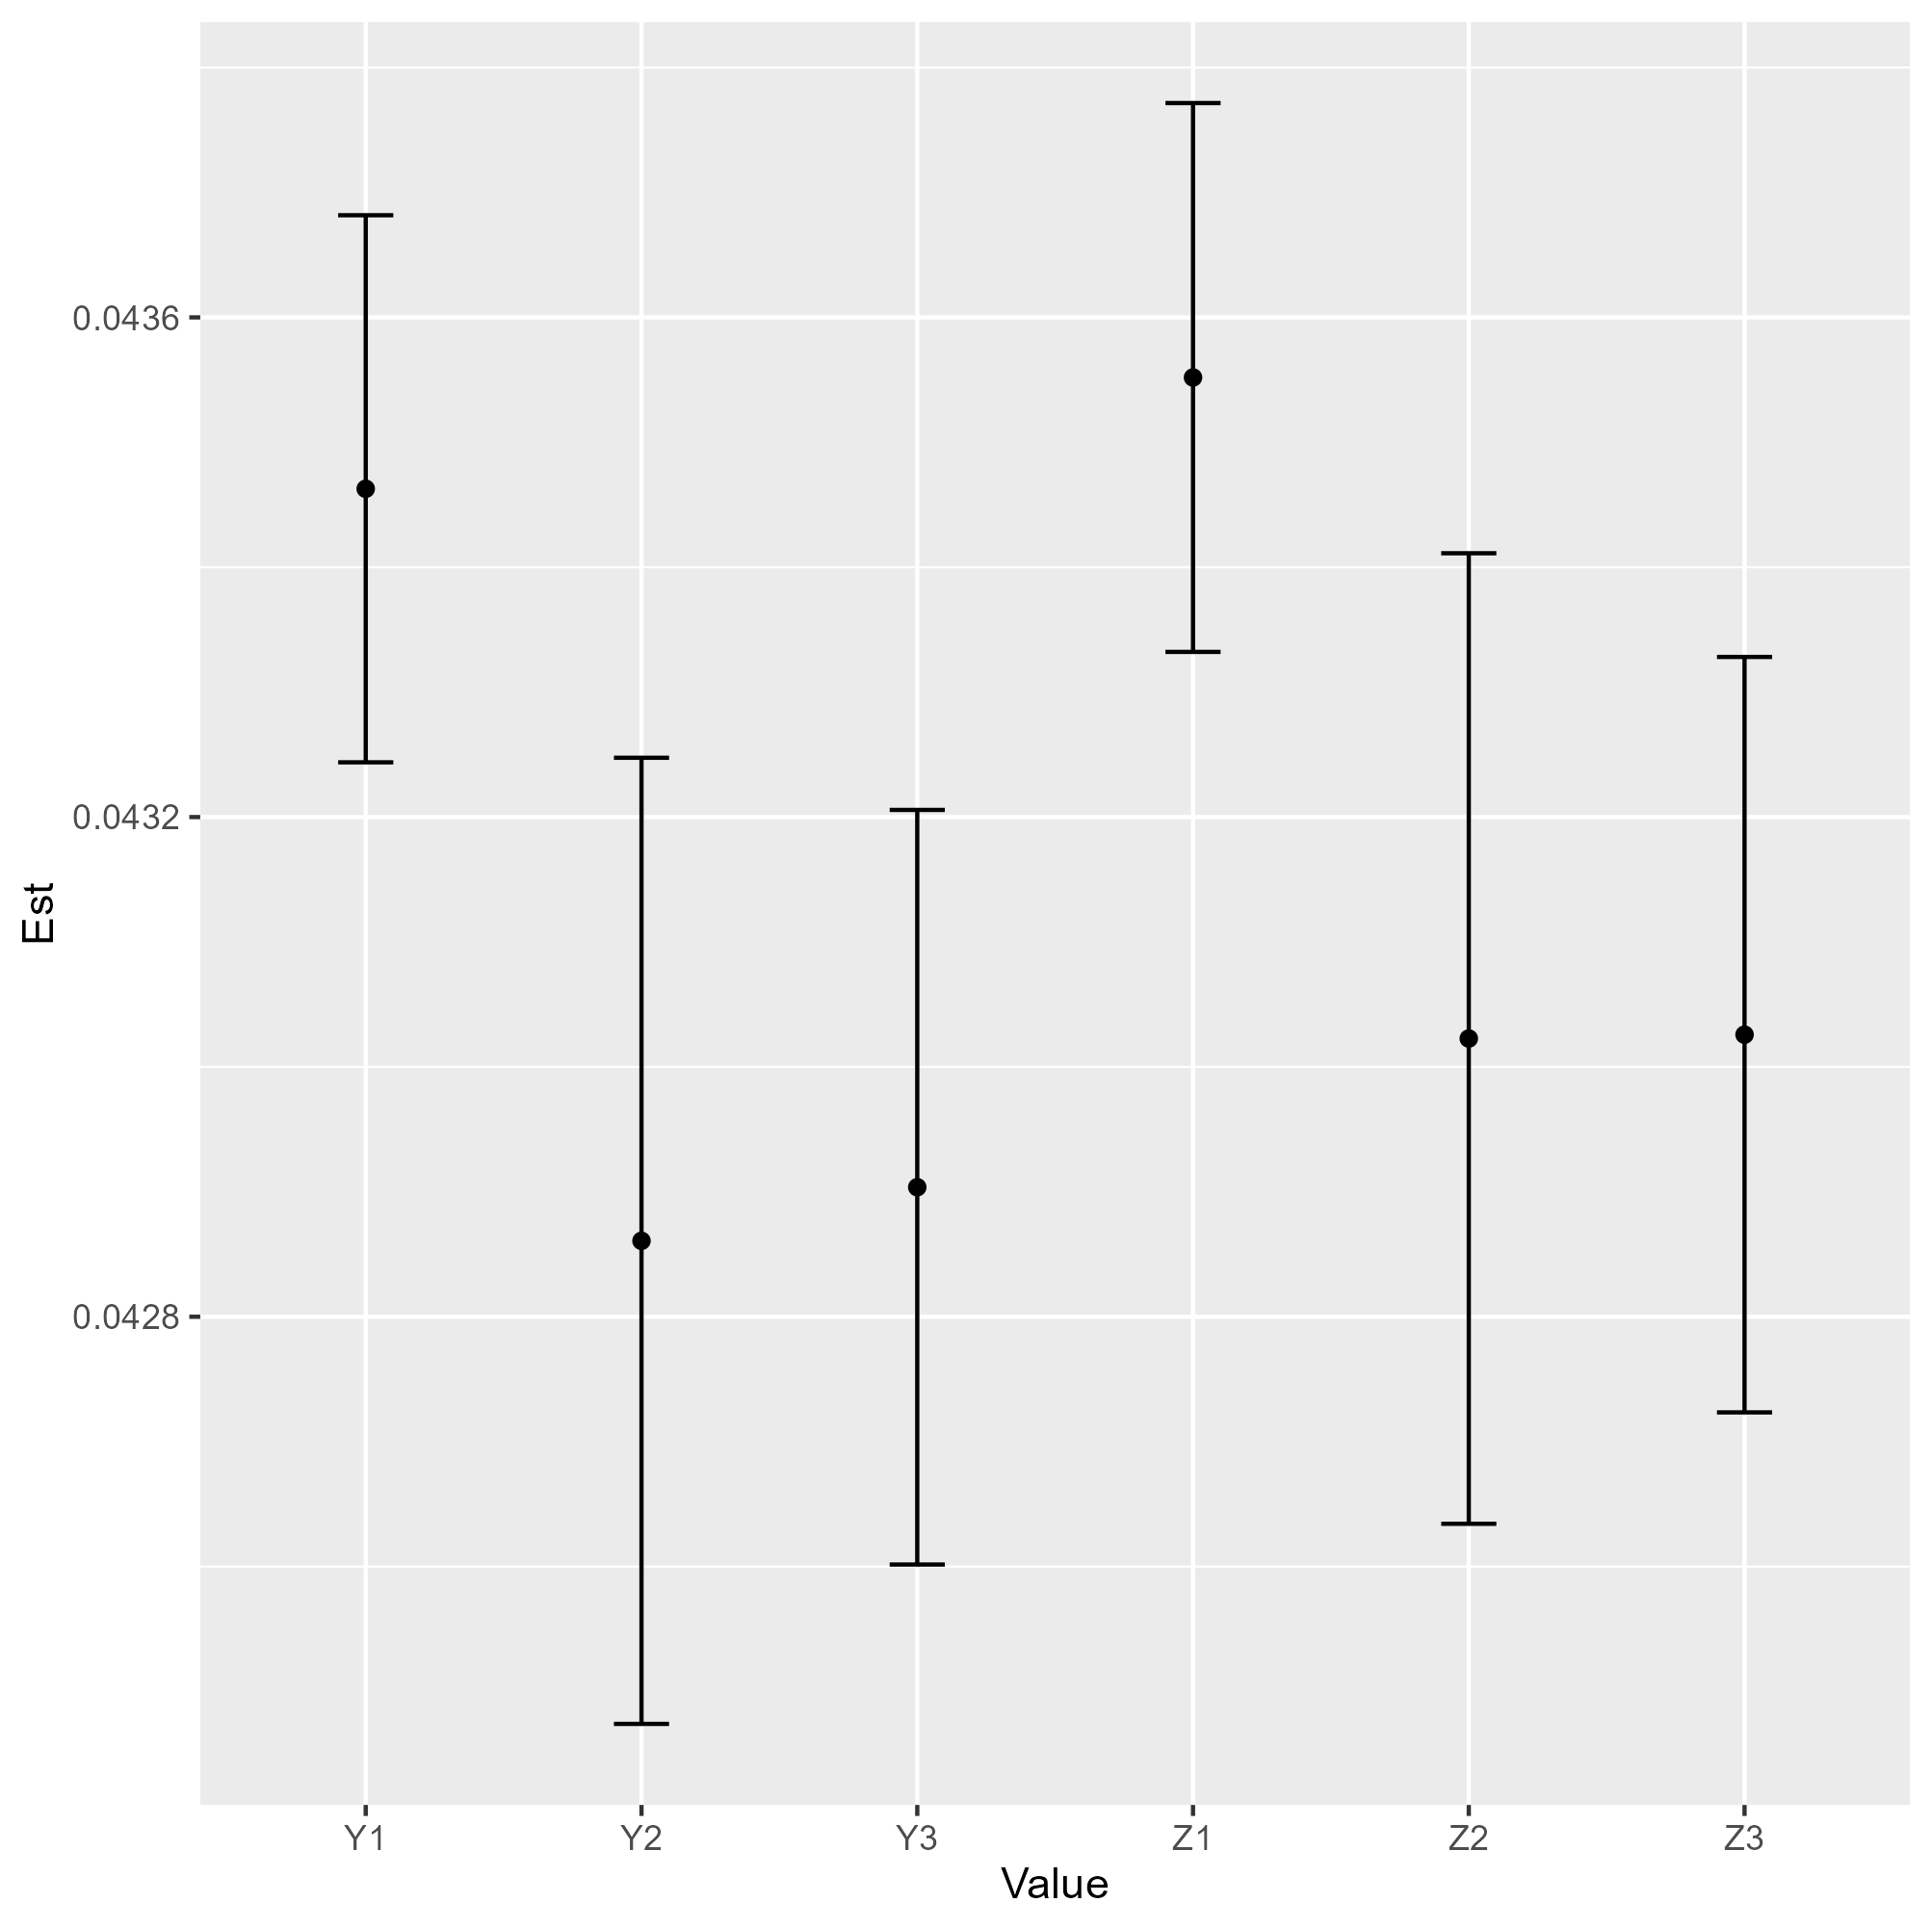
\includegraphics[width=4in]{Chap_6/Totals.png}
    \label{fig:Chap6_totals}
\end{figure}

\section{Spatial Sampling Designs}

So far, we have analyzed data that have already been collected.  However, ecologists are often responsible for defining and implementing a new sampling design, so we next turn to a brief review of spatial sampling designs and how they can affect spatio-temporal inference.

Sampling designs for ecological inference are quite varied, but can be classified as following a \myindex{probability sampling} design or not.  In a probability sampling design, a target population is divided into sampling units, where this set of sampling units is called a \myindex{sampling frame}.  Each sampling unit is then assigned a probability \( \pi_u \) of being included in a given sample, and then sampling proceeds to randomly select which sampling units to sample based on their assigned sampling probability \cite{cochran_sampling_1977}.  Spatial designs typically define the target population as a variable occurring within a spatial domain \(s \in \mathcal{D}\).  A spatial design then involves dividing this domain into sampling units that are defined geographically, where this set or union of sampling units then represents the sampling frame.  A spatial probability design would then assign a sampling probability to each unit.  We further categorize ecological sampling designs in Table \ref{tab:Chap6_sampling_designs}.  As noted there, simple and stratified random designs are types of probability sampling, while systematic and cluster sampling sometimes involve a probability design and sometimes do not, and opportunistic sampling generally does not.  We note that the sampling designs in Table \ref{tab:Chap6_sampling_designs} are not mutually exclusive.  For example, a stratified random design might include simple random sampling in one stratum and systematic sampling in another.  Similarly, a systematic design might involve sampling fish densities, and these densities might then be subsampled using a simple or stratified random design based on attributes of the captured individuals to measure characteristics like sex, age, and body size.  Multi-stage designs such as this then includes elements of multiple designs. 

\begin{table} 
  \caption[Categorizing ecological sampling designs]{A brief summary of common ecological sampling designs}
\begin{center}
\begin{tabularx}{\textwidth}{ | X m{4.25in} | } 
  \hline
  Sampling design & Description \\ 
  \hline

  Simple random & A type of probability sampling where all sampling units \(S_i\) in the sampling frame have an equal inclusion probability.  In this case, a design-based estimator for the population mean simply involves calculating the mean of those samples, and similarly, the squared standard error is the sample variance divided by the number of samples \\ & \\ 
  
  Stratified random & An extension of simple random sampling, where the spatial domain is divided into multiple non-overlapping sub-populations, defines a sampling frame for each sub-population (called \myindex{sampling strata}), and then applies simple random sampling within each sampling stratum.  A design-based index is then calculated for each stratum individually, where the total is the sum of design-based indices for each stratum, and the squared standard error is the sum of squared SEs for each stratum  \\ & \\ 
  
  Systematic & Defining an order for sampling units and then sampling at some pre-defined frequency along that order.  If sampling units are ordered spatially, then systematic sampling ensures that samples are evenly spread across space and thereby can improve sampling precision in some cases.  However, a different set of design-based estimators are appropriate to calculate the population mean and standard error  \\ & \\ 

  Fixed station (a.k.a. \textit{panel}) & Identifying a set of sampling units that are repeatedly sampled over time.  In this case, inference from samples to the population presumably requires that the fixed stations are representative, or that they are rotated periodically following a probability design (sometimes called a \textit{rotating panel design}).  In other cases, ecologists might select sites such that they can be intensively studied over time, and processes at each site are assumed to be representative of ecological processes in general, e.g., how inference is made from Long-Term Ecological Research network sites to global ecological processes \\ & \\

  Two-stage (or multi-level) & When sampling the density of a population that is highly clustered, ecologists often conduct some probability or systematic sample for primary sampling units across the entire sampling frame, and then conduct secondary sampling in secondary sampling units within those primary units.  For example, secondary sampling might be higher in the vicinity of individuals detected in the first stage.  Design-based estimators typically involve calculating the mean and variance in each primary sampling unit based on secondary sampling, and applying an estimator across primary sampling units \\ & \\

  Opportunistic & Analyzing data that arise from some process that the analyst does not control and hence cannot randomize (or perhaps even fully document).  For example, continuous-plankton records \cite{colebrook_continuous_1978} have been collected opportunistically on ocean-going vessels for many decades, and the Christmas Bird Count has involved citizen-scientists sampling birds \cite{bock_christmas_1981}. In general, there is no design-based estimator for these data that do not follow a design, so inference has historically involved proposing a model and using model-based inference \cite{butcher_evaluation_1990} \\
  
  \hline
\end{tabularx}
  \label{tab:Chap6_sampling_designs}
\end{center}
\end{table}

\begin{figure}[!ht]
    \caption[Sampling locations in simulated sampling designs]{The location of samples for a single replicate of the simulation design, arising from simple-random, stratified-random, or opportunistic sampling, where the latter has inclusion probability that is proportional to human population density.}
    \centering
    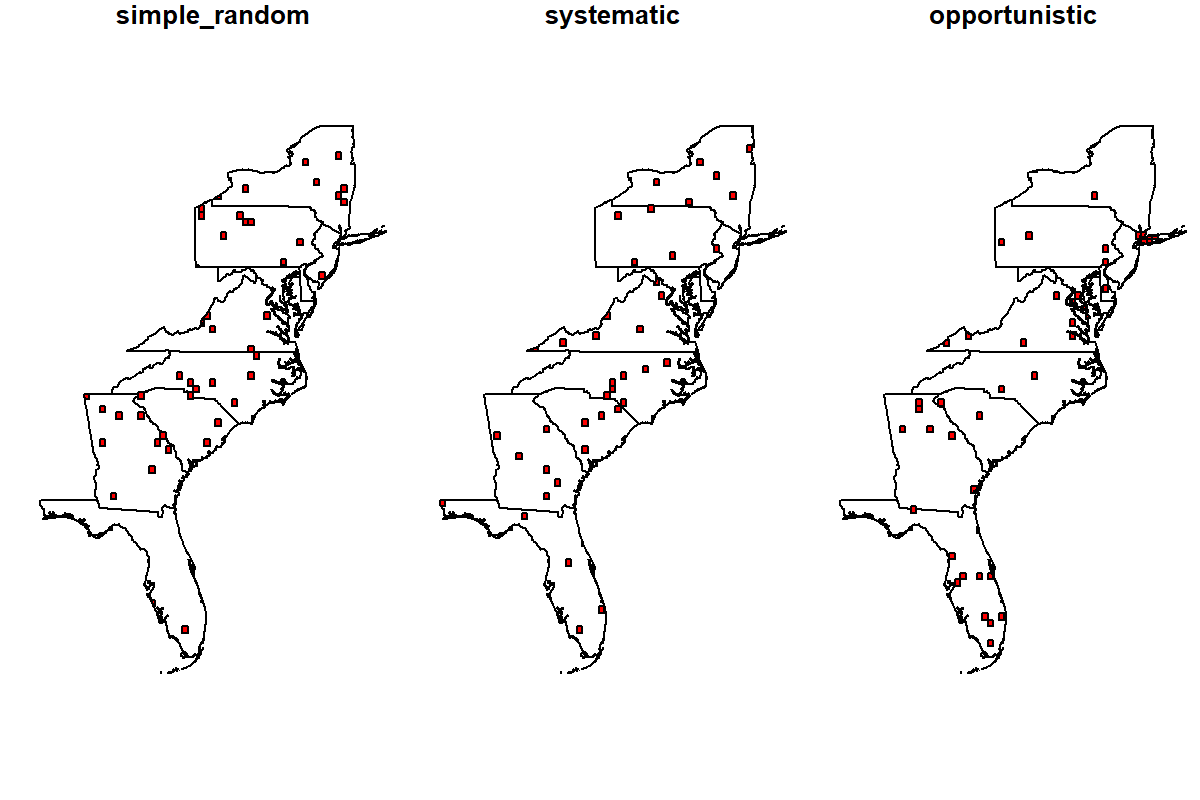
\includegraphics[width=5.5in]{Chap_6/Design.png}
    \label{fig:Chap6_design}
\end{figure}

We will illustrate these alternative sampling designs by simulating new data from the fitted ozone-concentration model analyzed previously, and then refitting the estimation model to simulation replicates.  We specifically apply three spatial sampling designs, each involving \(n_i=50\) measurements of ozone:
\begin{enumerate}
    \item \textit{Simple random sampling}, where each modeled location has equal chance of being sampled;

    \item \textit{Systematic sampling} based on the numbered sequence of grid cells, such that samples are distributed evenly across the spatial domain;

    \item \textit{Opportunistic sampling}, where inclusion probability \(\pi_g = a_g d_g\) is higher in grid cells with higher human population sizes (calculated as the product of population density and grid-cell area) in this example. 
\end{enumerate}
We then simulate data for 100 simulation replicates.  For each simulation replicate, we simulate a new value of the spatial variable \(\omega\) from its distribution when using maximum-likelihood estimates of fixed effects obtained when fitting to real-world data.  We then simulate new data at selected sampling units according to their probability in each sampling design.  An example of sampling locations (Fig \ref{fig:Chap6_design}) arising under each design confirms that systematic sampling results in samples that are distributed broadly across space, but also results in diagonal bands of closely packed samples where the sample spacing is similar to the number of cells in the dimensions of a given state, while opportunistic sampling results in dense sampling near New York City, Atlanta, Orlando, and other major urban areas.  

\begin{figure}[!ht]
    \caption[Errors in simulation experiment with alternative sampling designs]{Boxplots showing errors when estimating area-weighted average ozone concentrations using a log-linked spatial model fitted to data arising from simple-random, stratified-random, or opportunistic sampling and using either a plug-in estimator or epsilon bias-correction, where a well-performing model would have average error approaching zero (horizontal grey line). Note that the opportunistic sampling design has inclusion probability that is proportional to human population abundance (\textit{preferential sample}), which is expected to result in bias.}
    \centering
    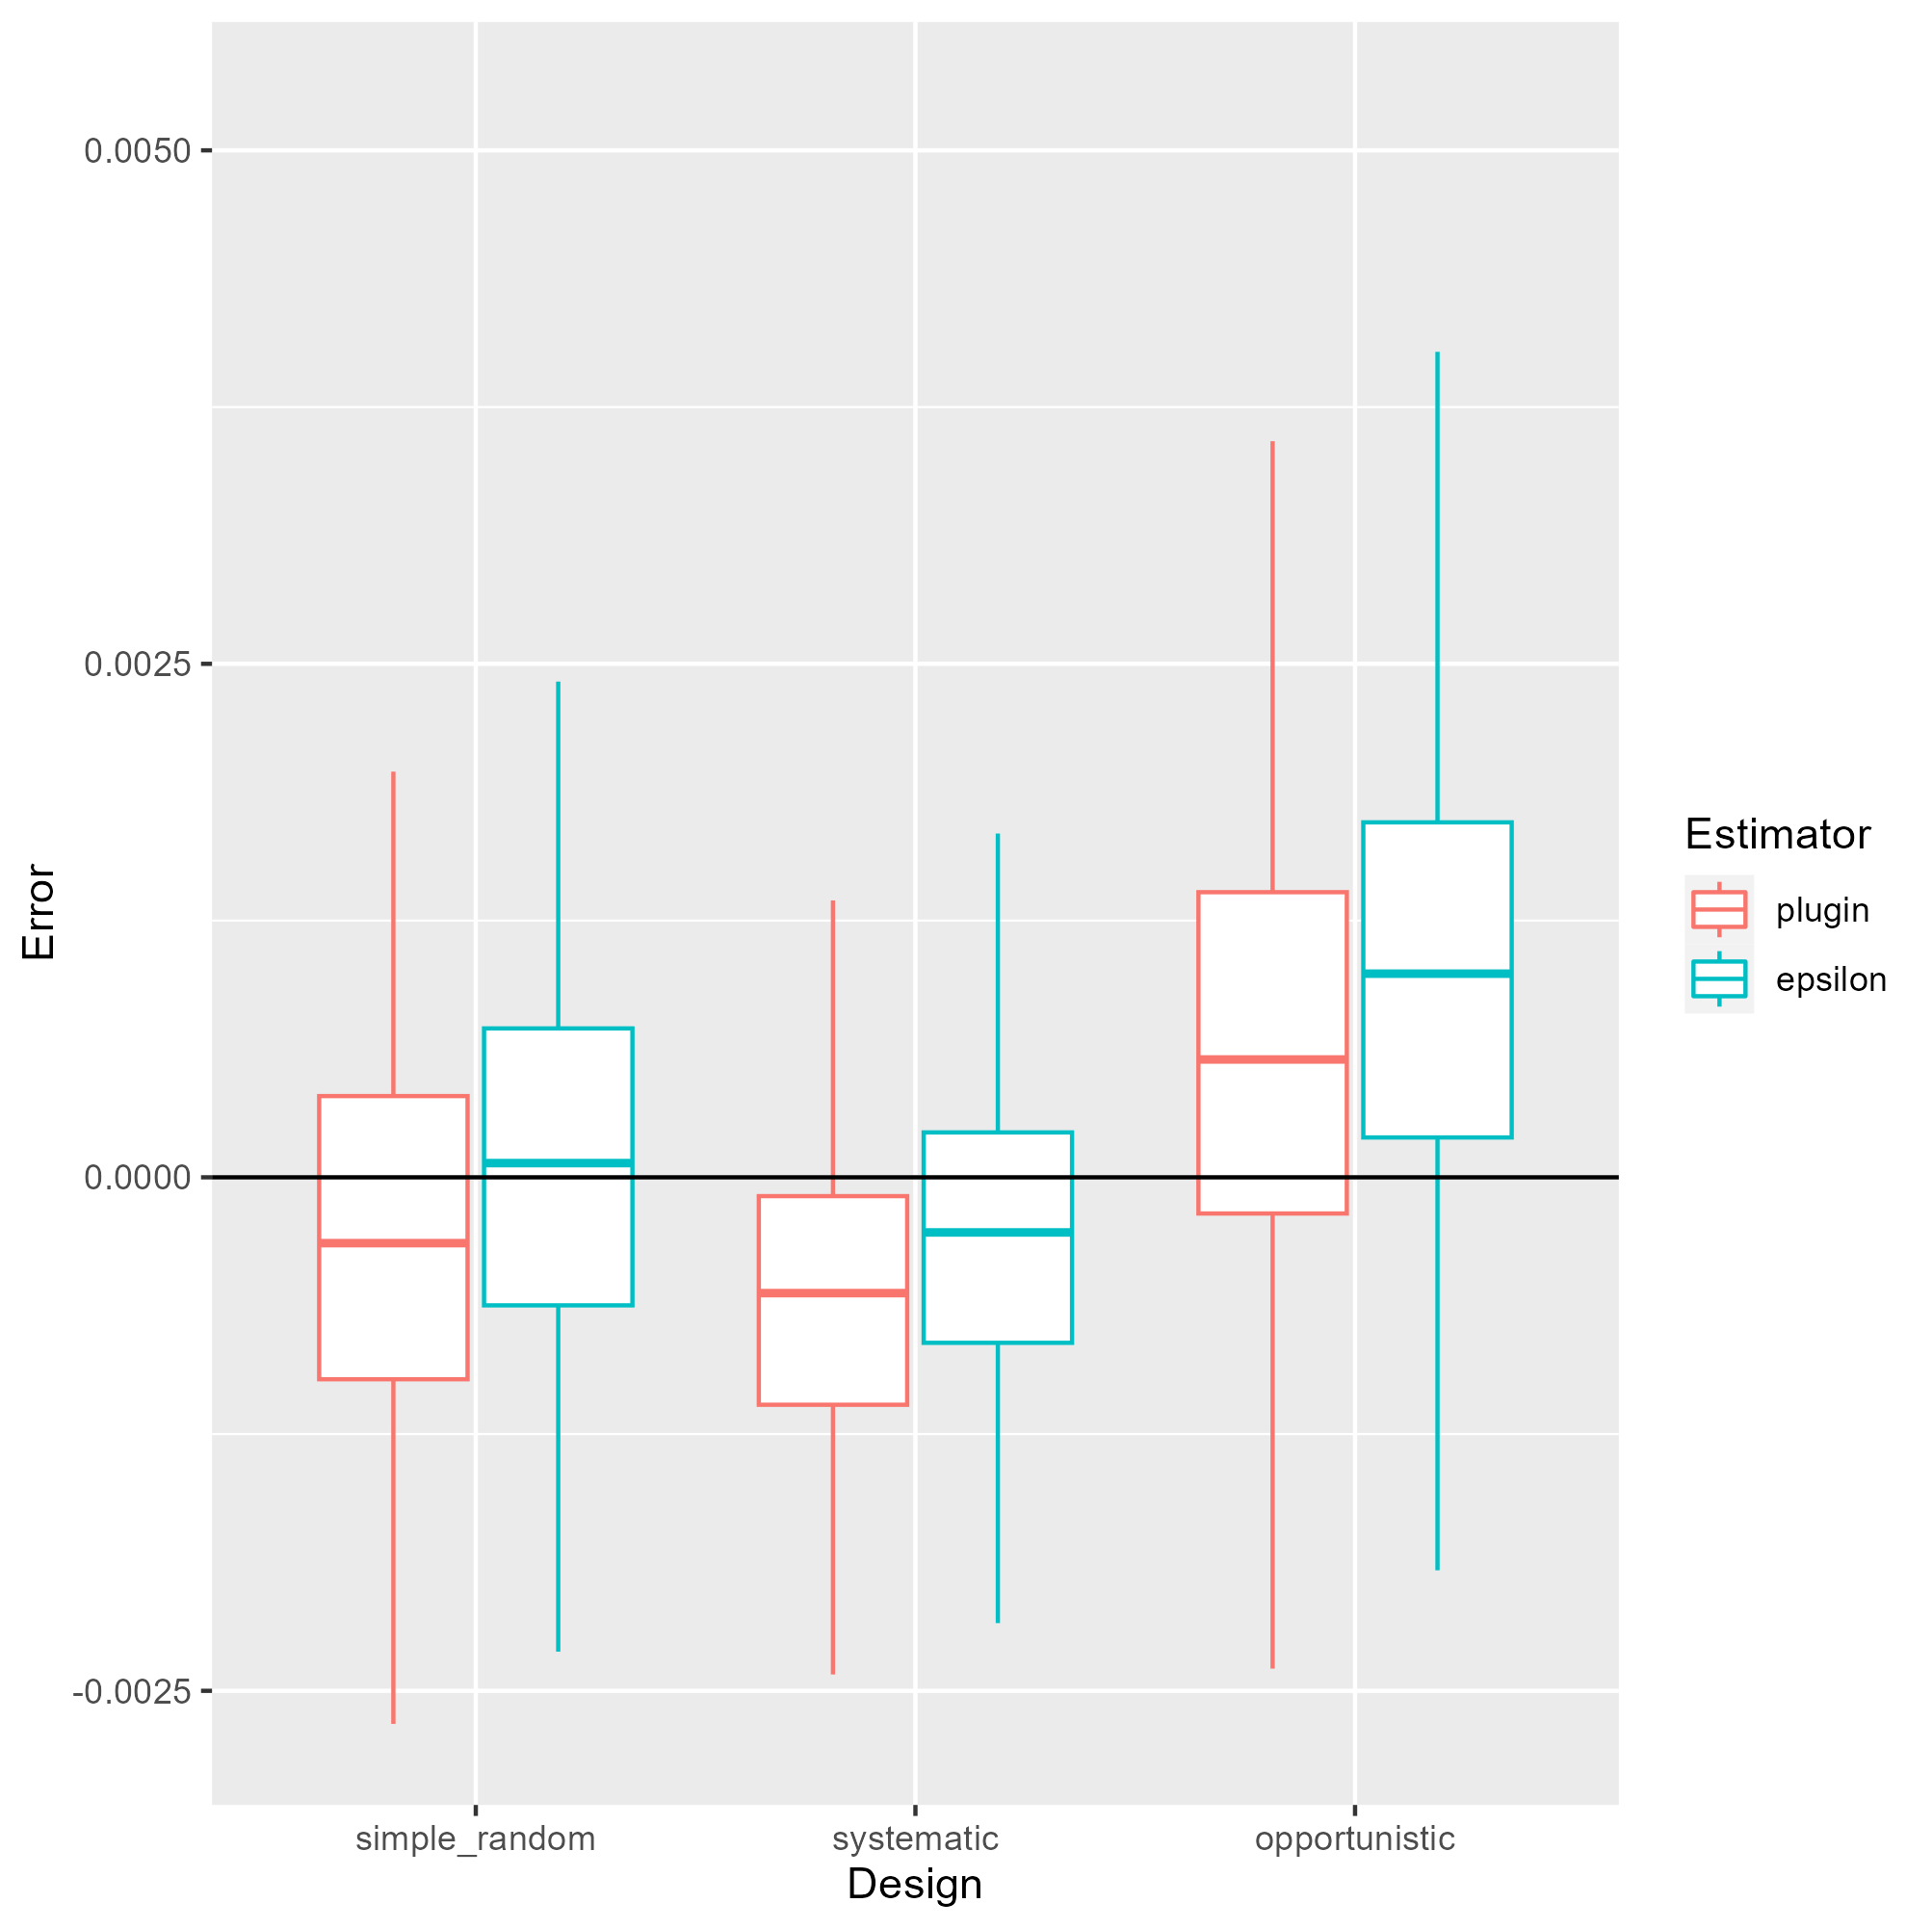
\includegraphics[width=4in]{Chap_6/Design_errors.png}
    \label{fig:Chap6_design_errors}
\end{figure}

For each replicate and design, we record the true area-weighted ozone concentration.  We then refit the estimation model while applying epsilon bias-correction to estimate area-weighted ozone concentrations.  We calculate error as the difference between estimated and true area-weighted ozone concentration, and plot the range of errors for each sampling design and also when comparing plug-in and epsilon bias-corrected estimates.  

This experiment illustrates several points (Fig. \ref{fig:Chap6_design_errors}).  First, the bias-corrected estimator is slightly higher than the plugin estimator for all designs, as expected given that we apply a log-linked linear model.  Second, analyzing data from the simple-random sampling design and applying the epsilon estimator results in estimates that are (approximately) unbiased. Meanwhile, the stratified design results in estimates that have a slight negative bias, while the opportunistic sampling design has a substantial positive bias.  The systematic design has smaller variation among replicates (i.e., more precision) than simple-random sampling, presumably due to the more even spread of sampling across space, and this increased precision appears to come at the cost of a slight negative bias.   Finally, the opportunistic design has a large positive bias, e.g., it generally estimates a higher area-weighted ozone concentration than actually holds in a given simulation replicate.  We discuss this bias in detail next.  

\section{Preferential Sampling} \label{sec:Chap6_preferential_sampling}

As seen in the simulation experiment (Fig. \ref{fig:Chap6_design_errors}), the opportunistic sampling-design has a substantial positive bias.  This phenomenon is called \myindex{preferential sampling}, and it arises whenever the spatial variable \( \omega(s) \) at each location \(s\) is correlated with inclusion probability \( \pi(s) \) \cite{ conn_confronting_2017,diggle_model-based_2007}.  To see this, consider a case where inclusion probability and the target function \( \mu(s) \) both vary based on the set of covariates \(\mathbf Z\):

\begin{equation} \label{eq:Chap6_preferential_sampling}
\begin{gathered}
    \mathrm{logit}(\pi_i) = \mathbf Z_i \mathbf \gamma \\
    \log(\mu_i) = \mathbf X_i \mathbf \beta + \mathbf Z_i \mathbf \lambda \\
    y_i \sim g( \mu_i ) 
\end{gathered} 
\end{equation}
This can then result in \( \mathrm{logit}(\pi_i) \) being correlated with \( \log(\mu_i) \).  In this case, the sample average \( \sum_{i=1}^{n_i} y_i \) will have expectation equal to the weighted average of \( \mu_i \) weighted by \( \pi_i \), rather than the area-weighted average.  Similarly, we might then fit a spatial model without covariates:

\begin{equation} 
\begin{gathered}
    \log(\mathbf{\mu}) = \beta_0 + \mathbf{A \omega}  \\
    \mathbf{\omega} \sim \mathrm{Normal}( \mathbf{0, Q}_{spde}^{-1} ) \\
    y_i \sim g( \mu_i )
\end{gathered} 
\end{equation}
where \(\mathbf{A}\) is the projection matrix representing bilinear interpolation and \(\mathbf{Q}_{spde}\) is the precision matrix calculated using the SPDE method (see Section \ref{sec:Chap5_SPDE}).  In this case, the estimated intercept \( \beta_0 \) will reflect the sample average, and the prediction of the target variable \( \log(\mathbf{\mu}) \) will be shrunk towards that sample average. In our simulation experiment involving ozone concentrations, the opportunistic sampling scenario had higher inclusion probability in locations with high population density, and these areas also had higher ozone concentrations, hence fitting the spatial model for the opportunistic sampling scenario resulted in a positive bias.  

The easiest way to avoid this bias is by ensuring that data arise from some probability sampling design where inclusion probabilities are independent from the target variable, or to intercalibrate opportunistic data against such data.  However, these solutions are often not feasible at the spatial scales that arise in ecological analyses without larger resources than are available.  Therefore, research has also sought to identify model-based approaches to mitigate bias from preferential sampling.  One such approach is simply to extend the spatial model to include in the spatial model those variables that drive variation in inclusion probability:

\begin{equation} 
\begin{gathered}
    \mathrm {log}(\mathbf{\mu}) = \beta_0 + \mathbf{A \omega} + \mathbf Z(s) \mathbf \lambda  \\
\end{gathered} 
\end{equation}
Including this term then controls for the effect of covariate \(\mathbf Z\), and results in spatial variable \(\omega\) being uncorrelated with inclusion probability \(\pi(s)\).  

\begin{figure}[!ht]
    \caption[Errors with model-based approach for preferential sampling]{Boxplots showing errors when estimating area-weighted average ozone concentrations using a log-linked spatial model fitted to data arising from opportunistic sampling where inclusion probability is proportional to human population abundance, but now fitted with population abundance as a covariate in the spatial model (and again showing either a plug-in estimator or epsilon bias-correction and a grey line at zero errors). The decreased bias relative to the opportunistic design in Fig. \ref{fig:Chap6_design_errors} illustrates the benefits of the model-based approach to preferential sampling.}
    \centering
    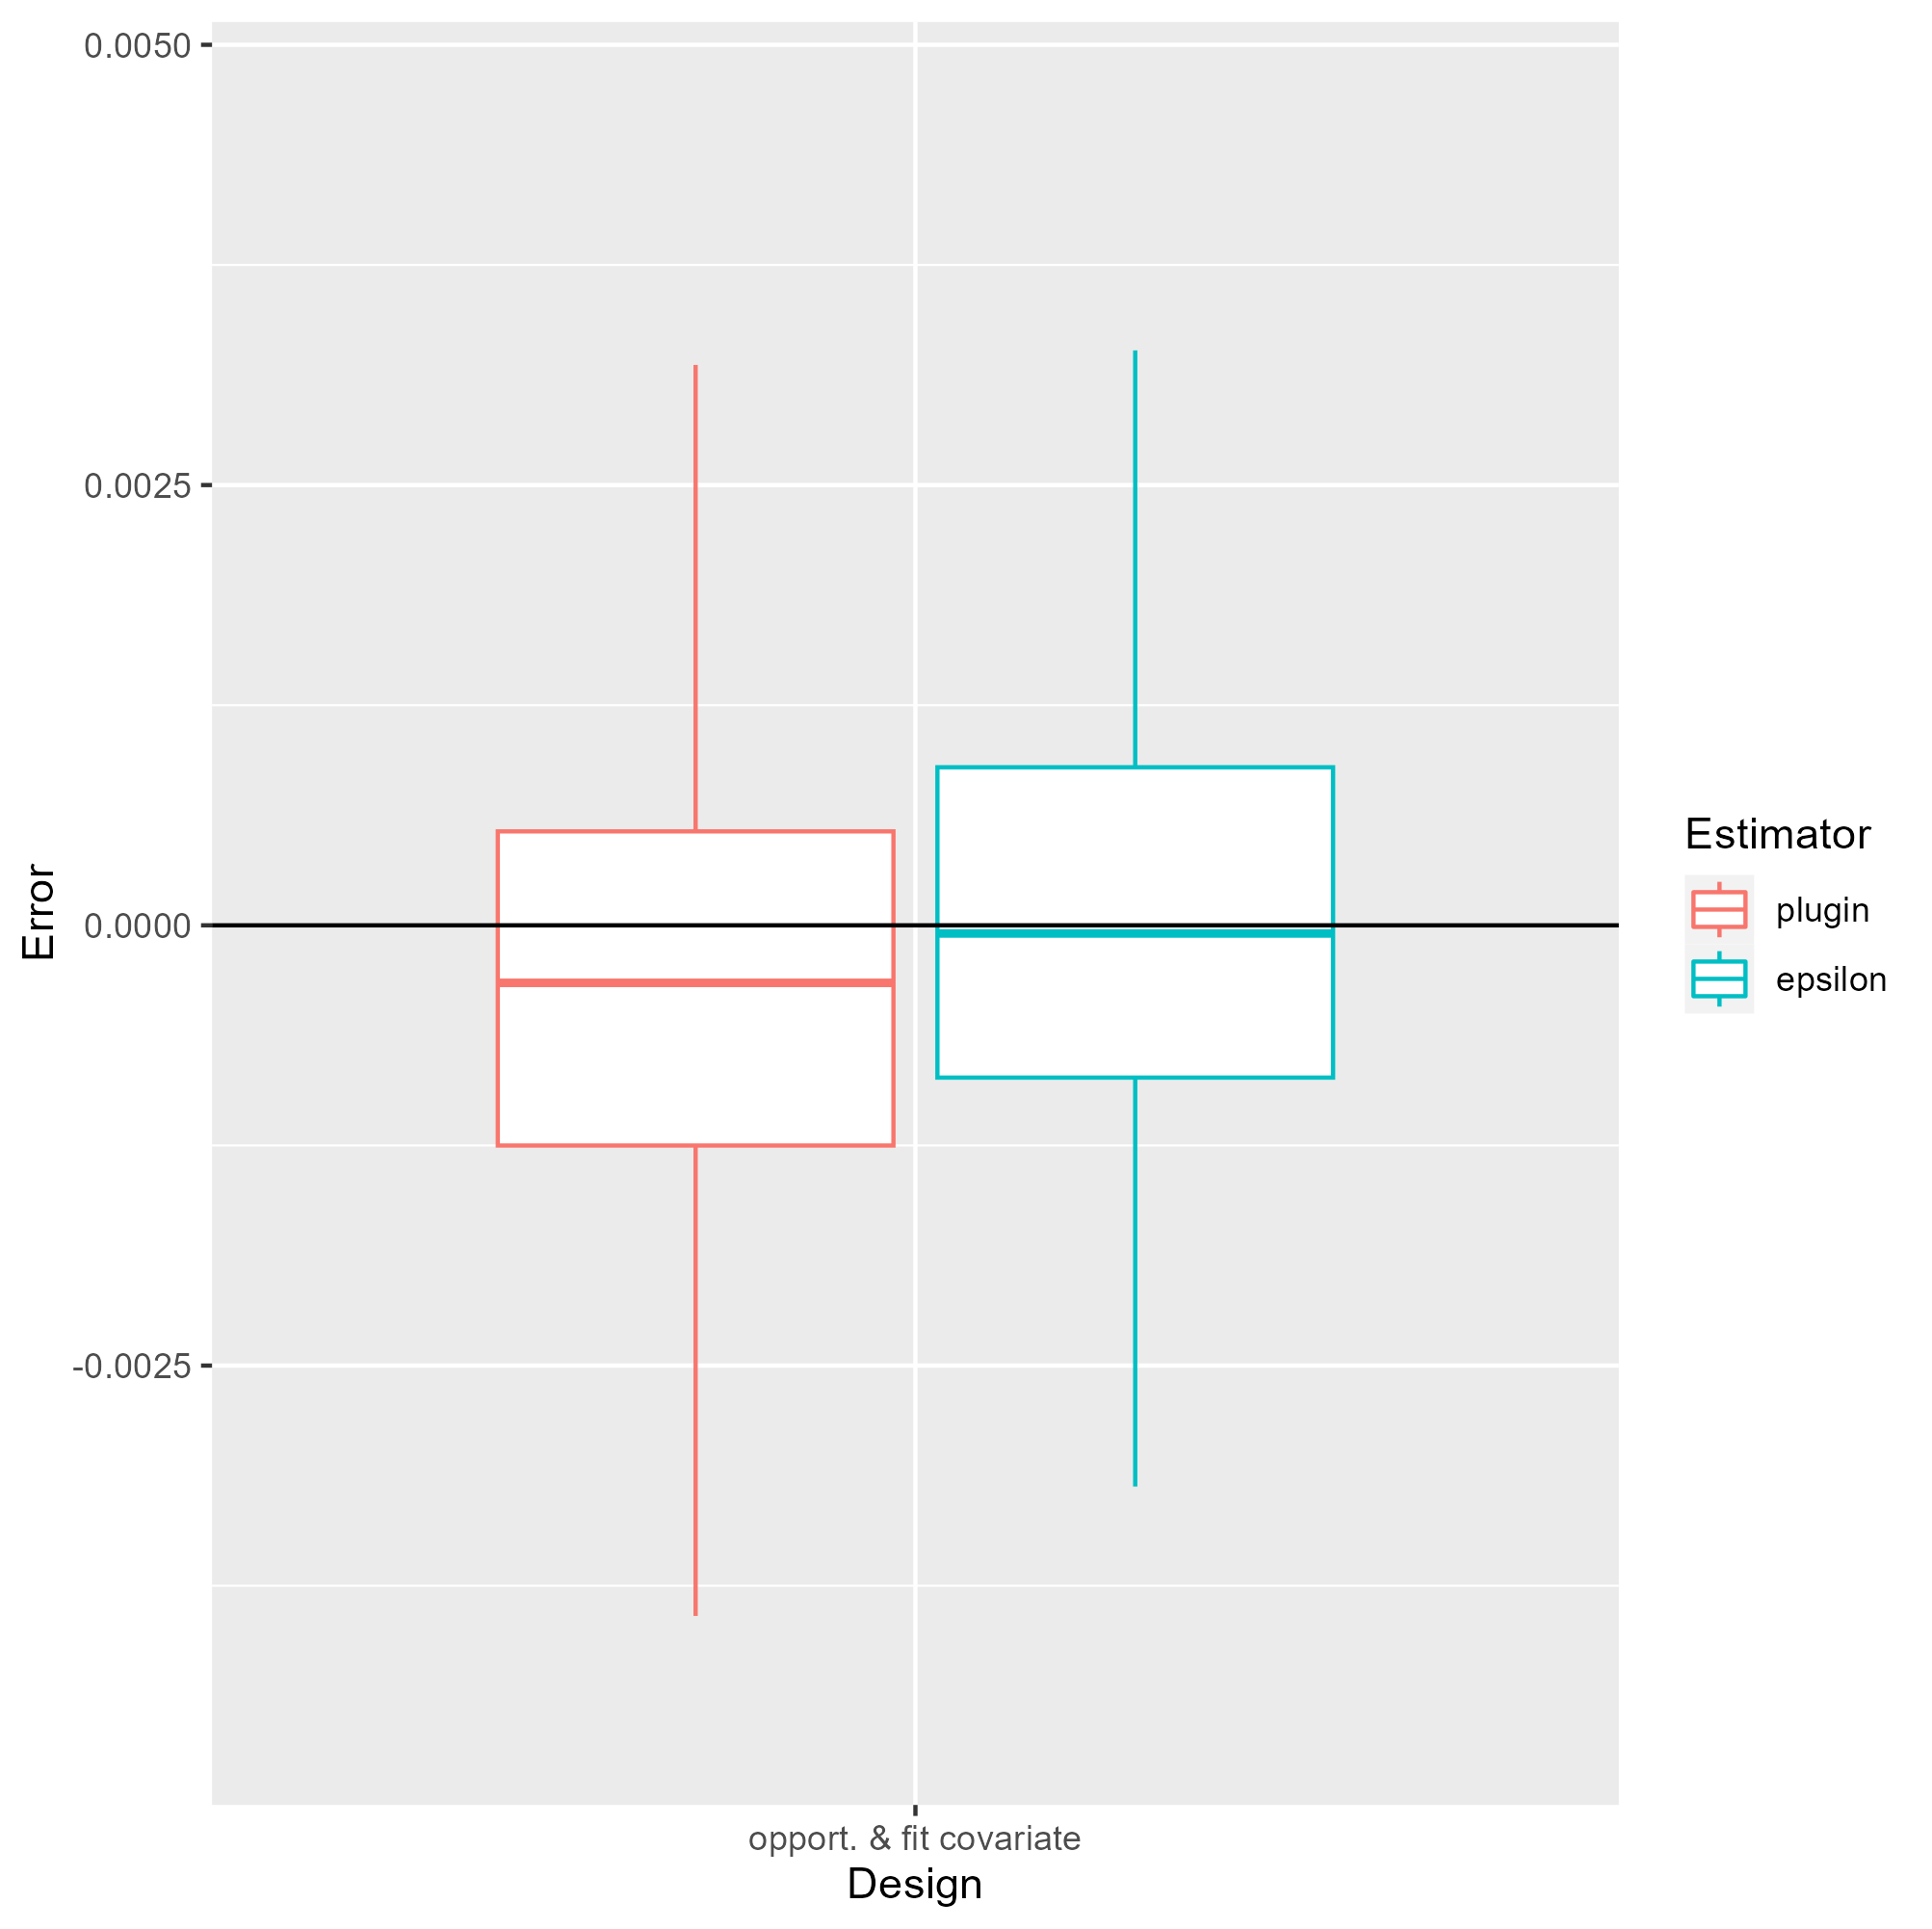
\includegraphics[width=4in]{Chap_6/Preferential_sampling.png}
    \label{fig:Chap6_preferential sampling}
\end{figure}

To demonstrate, we refit the ozone simulation experiment but including population density as a covariate in the spatial model.  In this case, the simulation and estimation models are perfectly matched, so we are unsurprised that the epsilon estimator results in an (essentially) unbiased estimate of area-weighted average ozone concentrations (Fig. \ref{fig:Chap6_preferential sampling}).  By contrast, the plug-in estimator has a small negative bias, presumably due to a failure to correct for retransformation bias.  Comparing these results with the other scenarios (Fig. \ref{fig:Chap6_design_errors}) shows that the model-based correction for opportunistic sampling results in somewhat larger interquartile range (i.e., boxplot width) and whiskers than the original model fitted to data arising from simple-random sampling.  This increased imprecision presumably arises due to the spatially clustered sampling arising from the opportunistic sampling scenario, as well as any uncertainty in the estimated preferential-sampling parameter \(\lambda\).  

\section{Multi-stage Sampling}

Finally, multi-stage sampling designs arise frequently in ecological systems, so we discuss them in greater detail here.  As an illustrative example, consider monitoring surveys in fisheries science, where ecologists typically use an established sampling protocol and gear consistently over large areas and several decades (i.e., a bottom trawl towed at a known speed for a fixed time) to obtain samples of fish abundance using a standardized unit of sampling effort.  Analysts then typically assume that this protocol catches a proportion of local abundance, where this proportion is called \myindex{detectability} or \textit{catchability}.  If this detectability or catchability is then assumed to be constant over time and space, then spatial and temporal variation in expected catch is proportional to changes in local densities.

However, ecologists then often want to estimate population-level attributes of those fishes, and proceed by measuring those attributes for sampled individuals.  For those individuals that are detected during a sampling design, an ecologist might conduct a subsample and for those subsampled individuals measure their age, body size, sex, maturation state, or their physiological condition (energy content, metabolic rates, stomach contents, etc.).  Fisheries monitoring therefore involves subsampling the total catch from each sampling event (i.e., dividing into randomized buckets on deck) and enumerating the species, size, age, or attributes of individuals in that subsample.  

\subsection{Estimators for Multi-stage Sampling}

 In this illustrative example, we call the original bottom-trawl set a \myindex{primary sampling unit}, where the sampling locations in a monitoring survey are typically randomized using a simple or stratified-random design with known inclusion probability.  The subsampled individuals are then \myindex{secondary sampling units}.  In our example, these secondary units are obtained using a simple-random sampling design while using the outcome of the primary unit as the sampling frame; the inclusion probability \(\pi_j\) for each individual in the secondary sampling is then equal to the fraction of the primary unit that is subsampled.  This multi-level design might continue onward to a tertiary sampling design, wherein individual fish have their stomachs removed, and only a simple random subsample of stomach contents is then enumerated to species.

The key insight in multi-stage sampling designs is that a secondary (or tertiary etc.) sampling unit has an inclusion probability that arises from the inclusion probabilities of each higher level in a given design.  For example, a primary sampling unit might have inclusion probability \( \pi_i \), and conditional on that unit being sampled a given fish might have inclusion probability \( \pi_j \), such that the unconditional probability of that fish being sampled is \(\pi_i \pi_j\).  For this reason, it is important to identify and account for mechanisms for preferential sampling occurring at all sampling level.  For example, subsampling fractions in a secondary sampling design often depend upon the outcome of the primary sampling unit;  a bottom trawl sample with 10 tonnes of fish will typically subsample a smaller fraction than a sample with only 10 kg (due to time-constraints for sorting each sample).  This then results in a lower unconditional inclusion probability for those individuals in high-density areas, and this variation in inclusion probability might be systematically correlated with species composition or size.  Ignoring this variation in unconditional inclusion probability then gives rise to preferential sampling bias, and as a result, it could yield biased inference about average age or size for the population as a whole (e.g., \cite{thorson_standardizing_2014}).

One simple solution to this scenario is to apply a separate and unbiased estimator to each level of the design.  This might involve taking a measurement from the secondary sampling unit, estimating the expected measurement if the entire primary sampling unit had been subsampled, and treating that estimate as data in a subsequent analysis of primary sampling units.  In our multi-level fisheries sampling design, for example, this might involve recording the count-at-age for a given species in a secondary sample, dividing this by the subsampling fraction to estimate the expected count-at-age if the entire tow had been subsampled, and then treating this expanded count-at-age as data in a subsequent model \cite{thorson_spatiotemporal_2018}.  

\subsection{Occupancy Models and Demographic Closure} \label{sec:Chap6_occupancy_model}

However, these concepts are more complicated when ecologists create a design where a sampling unit is repeatedly sampled over a short time-scale, such that the variable in each sampling unit is unlikely to change between samples.  When sampling abundance this assumption is often called \myindex{demographic closure}, because the sampling unit is closed to demographic changes like births, deaths, and migration during secondary sampling.  It is possible to interpret these multiple replicated measurements as secondary sampling units, average them to reduce sampling variance for the primary sampling unit, and proceed with spatial analysis as normal.  However, replicated samples given demographic closure can often yield additional useful information about detection probabilities.  

For example, consider the case that a given site has latent abundance \(N\), and we obtain \(J\) measurements of animal abundance \( \{ C_1, C_2, ..., C_J \} \).  Let's make several further assumptions:  (1) that the sampling unit is demographically closed during these replicated counts; (2) that each individual is randomly distributed and has probability \(q\) of being counted in each sample, where this probability is constant for all individuals and samples; and (3) each count does not mistakenly enumerate the same individual multiple times such that each count \(C_j\) follows a Binomial distribution with the same latent abundance and detectability.  These assumptions result in an \myindex{N-mixture model} \cite{royle_n-mixture_2004}, and we can then define the probability for these counts as:

\begin{equation} \label{eq:Chap6_Nmixture}
    \mathrm{Pr}( C_1, C_2, ..., C_J | N, q ) = \prod_{j=1}^J \mathrm{dBinomial}( C_j | N, q )
\end{equation}
where \(\mathrm{dBinomial}(C|N,p) = \frac{N!}{(N-C)!C!} p^C (1-p)^{N-C} \) is probability mass function for the Binomial distribution.  The marginal likelihood of detection probability is then approximated by marginalizing across latent abundance \(N\) from a specified lower to upper limit (e.g., lower limit \(L=\mathrm{max}(C)\) to upper limit \(U=200\)):

\begin{equation}
    \mathcal{L}( q; C_1, C_2, ..., C_J ) = \sum_{N=L}^{U} \mathrm{Pr}( C_1, C_2, ..., C_J | N, q )
\end{equation}
where the simulation below illustrates that this yields a biased but potentially useful estimator for detection probability \(q\).  

\lstset{style=Rcode}
\lstinputlisting[language=R, label=code:Chap6-Nmixture, caption=R code simulating an N-mixture estimate of detection probability., captionpos=t]{Chap_6/Nmixture_example.R}

Under the specified assumptions, the variance among samples can be used to define the variance of measurement errors.  To provide intuition, note that:

\begin{itemize}
    \item The sample variance of replicated counts \( \mathrm{Var}(C_1, C_2, ..., C_J) \) provides a measurement of the theoretical variance \(\mathrm{Var}(C)\) arising from a Binomial distribution \( C \sim \mathrm{Binomial}(N,q) \);
    
    \item As sampling captures all individuals in the demographically closed sampling unit (\( q \to 1 \)), each sample becomes a census and the sample variance among replicated measurements will vanish \( \mathrm{Var}(C_1, C_2, ..., C_J) \to 0 \);  

    \item As sampling captures a miniscule proportion of local individuals (i.e., \( q \to 0 \) and \( N \to \infty \)), then each sample will follow a Poisson distribution with intensity \( \E(C) = \lambda = qN \), such that the variance among replicates also approaches this value \( \mathrm{Var}(C_1, C_2, ..., C_J) \to \mathrm{mean}(C_1, C_2, ..., C_J) \);

    \item Intermediate values for detection probability will also result in intermediate values for among-sample variance (i.e., if \( 0 < p < 1 \) then \( 0 < \mathrm{Var}(C_1, C_2, ..., C_J) < \mathrm{mean}(C_1, C_2, ..., C_J)\), where the function relating among-sample variance \( \mathrm{Var}(C_1, C_2, ..., C_J) \) to detection probability is monotonic and decreasing.
\end{itemize}
The variance among replicated samples \( \mathrm{Var}(C_1, C_2, ..., C_J) \)  therefore provides information that is useful to estimate detection probabilities \(q\).  More formally, we can compute the expected variance and expected mean:

\begin{equation}
\begin{gathered}
   \E(C) = qN \\
   \mathrm{Var}(C) = q(1-q)N
\end{gathered}    
\end{equation}
such that their ratio \( \frac{\mathrm{Var}(C)}{\E(C)} = 1-q \).  Therefore the ratio of the sample variance and sample mean is an estimator for the probability of not detecting each individual.  We note that a similar model can be derived when measuring whether each sampling unit is occupied or unoccupied, and this is conventionally called an \myindex{occupancy model} \cite{mackenzie_occupancy_2005}.  Both occupancy and N-mixture models can then be modeled with abundance or occupancy varying between primary sampling units, although this still requires that each primary sampling unit is demographically closed during replicated sampling.  

This N-mixture model \cite{royle_n-mixture_2004} can then be used in place of other estimators for secondary sampling units, and a spatial model used to extrapolate density based on primary sampling units \cite{goldstein_comparing_2022,thorson_demographic_2014}.  However, we recommend extreme caution when using the among-sample variance of secondary sampling units to infer detection probabilities, because the estimate of detection probability can be biased due to even mild violations of the assumptions listed previously \cite{rota_occupancy_2009}.  

\section{Chapter Summary}

In summary, we have showed that:
\begin{enumerate}
    \item Inference about regional patterns involves spatial integration.  This can be implemented by identifying integration points, predicting variables at those locations, and then aggregating across integration points.  This spatial integration can be weighted in many different ways, including sample, area, covariate, and multivariate-weighting methods, and these typically correspond to different types of ecological inference.  For example, population abundance typically requires area-weighting, calculating per-capita exposures requires covariate weighting, and measuring average demographic rates requires density-weighting (a type of multivariate weighting);

    \item Ecologists often estimate quantities that result from both fixed and random effects (e.g., total abundance where densities arise from spatially correlated random effects).  In these cases, a simple ``plug-in" estimator will be subject to \textit{retransformation bias}, where this bias increases with the nonlinearity of the transformation as well as the uncertainty and skewness of random effects.  These biases can be largely mitigated using the \textit{epsilon estimator}, which involves calculating the gradient of an expanded form of the marginal likelihood with respect to the derived quantity;  

    \item Analysts should estimate, visualize, and communicate uncertainty in density predictions.  Uncertainty in derived quantities can be calculated from the joint precision matrix of fixed and random effects, either using the generalized delta method or a sample-based approximation.  The sample-based method introduces additional sampling error, but does not substantially increase computational time even for a large number of uncertainty calculations.  Therefore, choosing between these two methods depends upon analytical goals and context;  

    \item Ecologists often specify a sampling design that results in new data. Designs can be categorized as following probability sampling or not, and further categorized as simple or stratified-random sampling, systematic or fixed-station sampling, two-stage (cluster) sampling, and opportunistic sampling.  These designs represent a trade-off between sampling efficiency and potential bias where, e.g., systematic sampling can spread data more evenly and reduce standard errors when applying a spatial model.  Each of these can be specified to include replicated sampling during a short time interval that is closed to demographic changes, and in this case the sampling variance is sometimes informative about detection probabilities;

    \item If sampling rates (``inclusion probabilities") are correlated with the variable being modeled (termed ``preferential sampling"), then a standard spatial model will result in biased inference about regional averages.  This bias can sometimes be mitigated by including additional covariates or random effects that explain the variation in sampling intensity within the spatial model for a target variable.  
\end{enumerate}

\section{Exercises}

\begin{enumerate}
    \item In Section \ref{sec:Chap6_occupancy_model}, we defined an N-mixture model by specifying a Bernoulli distribution for replicated samples of a primary sampling unit that is demographically closed.  We then provided Code \ref{code:Chap6-Nmixture}, which showed how to simulate samples from this model for a single primary sampling unit, and then marginalize across local abundance to calculate the likelihood function for estimating detectability.  Please expand this code to simulate abundance and replicated samples for 20 primary sampling units (sites), where site each has local abundance drawn from a Poisson distribution \(N_i \sim \mathrm{Poisson}(\lambda=20)\) and has three replicated samples.  Then, expand the estimation model (either in R or TMB) to include the same Poisson distribution for local abundance, now estimating two parameters, detectability \(q\) and average density \(\lambda\).  Please use a simulation experiment to explore the performance for estimating detectability and average density when varying four inputs: the true values for these two parameters, as well as the number of sites and the number of replicated samples per site.  For each of these four experimental axes, please identify whether increasing its value increases or decreases the precision for estimates of detectability and average density.

    \item In Section \ref{sec:Chap6_preferential_sampling}, we showed that we can mitigate bias arising from opportunistic sampling when the inclusion probability \(\pi(s)\) is correlated with the random variation in the target variable \(\omega(s)\).  Please expand the code used for the simulation experiment in that section to also apply the preferential sampling estimator (Eq. \ref{eq:Chap6_preferential_sampling}) to simple random and systematic scenario sampling scenarios.  What is the distribution for estimates of the parameter \(\lambda\) linking inclusion probability to target variable density?  How does estimating this extra parameter affect the precision and bias for the total area-weighted ozone concentration?

\end{enumerate}


